% !TEX encoding = UTF-8 Unicode
%!TEX TS-program = xelatex

\documentclass[12pt]{extarticle}
% extarticle is like article but can handle 8pt, 9pt, 10pt, 11pt, 12pt, 14pt, 17pt, and 20pt text

\def \ititle {Origins of Mind}
 
\def \isubtitle {Lecture 08}
 
\def \iauthor {Stephen A. Butterfill}
\def \iemail{s.butterfill@warwick.ac.uk}
\date{}

%for strikethrough
\usepackage[normalem]{ulem}

\usepackage{pdfpages}


\input{$HOME/Documents/submissions/preamble_steve_handout}

%logic symbol \leftmodels
\usepackage{MnSymbol}

%\bibpunct{}{}{,}{s}{}{,}  %use superscript TICS style bib
%remove hanging indent for TICS style bib
%TODO doesnt work
\setlength{\bibhang}{0em}
%\setlength{\bibsep}{0.5em}


%itemize bullet should be dash
\renewcommand{\labelitemi}{$-$}

\begin{document}

%\raggedcolumns

\begin{multicols*}{3}

\setlength\footnotesep{1em}


\bibliographystyle{newapa} %apalike

%\maketitle
%\tableofcontents




%--------------- 
%--- start paste

\def \ititle {Logic (PH133)}
 
\def \isubtitle {Lecture 6}
 
\begin{center}
 
{\Large
 
\textbf{\ititle}: \isubtitle
 
}
 
 
 
\iemail %
 
\end{center}
 
Readings refer to sections of the course textbook, \emph{Language, Proof and Logic}.
 
 
 
\section{DeMorgan: ¬(A ∧ B) $\leftmodels\models$ ¬A ∨ ¬B}
 
\emph{Reading:} §3.6, §4.2
 
`$\leftmodels\models$' means `is logically equivalent to', so for now `has the same truth table as'.
 
A $\leftmodels\models$ ¬¬A
 
¬(A ∧ B) $\leftmodels\models$ (¬A ∨ ¬B)
 
¬(A ∨ B) $\leftmodels\models$ (¬A ∧ ¬B)
 
A → B $\leftmodels\models$ ¬A ∨ B
 
¬(A → B) $\leftmodels\models$ ¬(¬A ∨ B) $\leftmodels\models$ A ∧ ¬B
 
 
 
\section{Negation and the arrow: A → ¬B $\nvDash$ ¬(A → B)}
 
\emph{Reading:} §3.6
 
\begin{center}
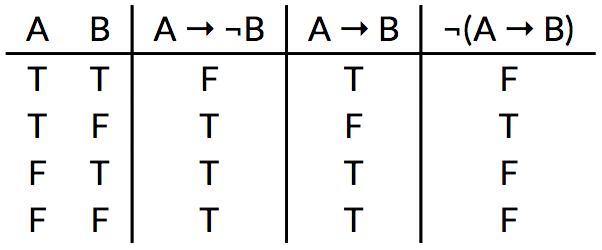
\includegraphics[scale=0.3]{img/unit_237_tt.png}
\end{center}
 
 
\section{Don't use ∃ with →}
 
\begin{minipage}{\columnwidth}
 
Is true ∃x(Square(x) → Broken(x)) in this world?
 
\begin{center}
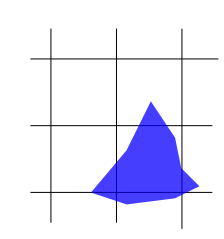
\includegraphics[scale=0.3]{img/word_02.png}
\end{center}
\end{minipage}
 
∃x(Square(x) → Broken(x))
 
\hspace{3mm} $\leftmodels\models$
 
∃x(¬Square(x) ∨ Broken(x))
 
\hspace{3mm} $\leftmodels\models$
 
∃x(¬Square(x)) ∨ ∃x(Broken(x))
 
 
 
\section{¬Intro}
 
\emph{Reading:} §5.3, §6.3
 
\begin{center}
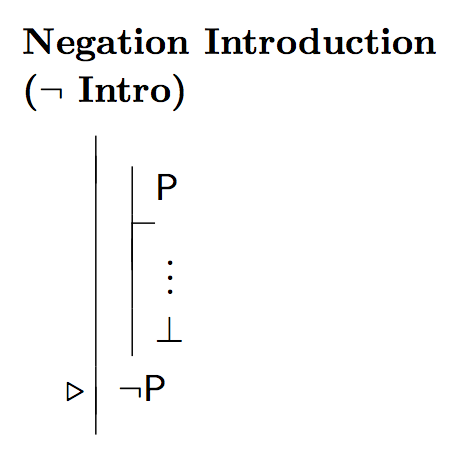
\includegraphics[scale=0.3]{img/rule_negation_intro.png}
\end{center}
\begin{center}
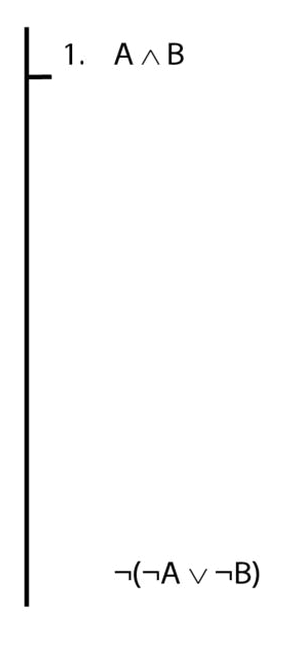
\includegraphics[scale=0.3]{img/proof_example_unit_281.png}
\end{center}
 
 
\section{¬Intro Proof Example}
 
\emph{Reading:} §5.3, §6.3
 
\begin{center}
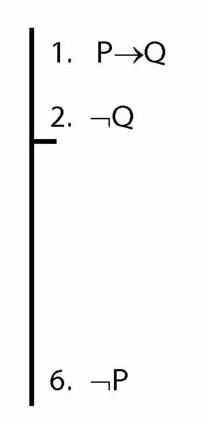
\includegraphics[scale=0.3]{img/unit_283_proof.png}
\end{center}
 
\columnbreak 
\section{Subproofs Are Tricky}
 
What is wrong with the following apparent proof?
 
\begin{center}
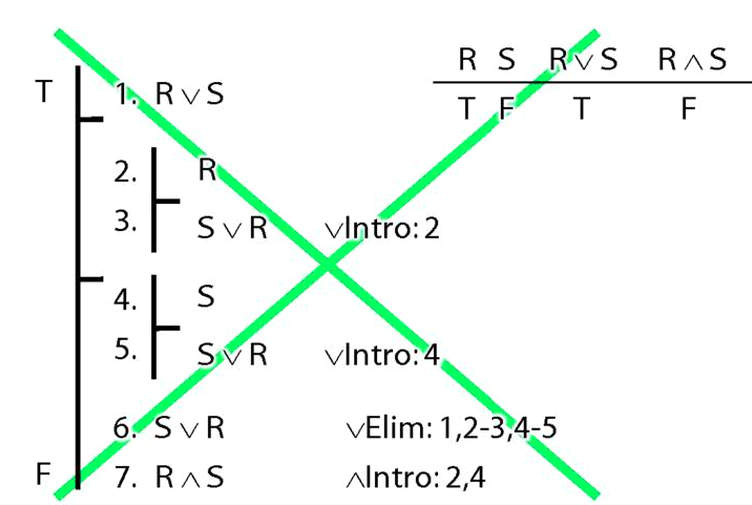
\includegraphics[scale=0.3]{img/unit_224_subproofs_tricky.png}
\end{center}
 
 
\section{∀Elim}
 
\emph{Reading:} §13.1
 
\begin{center}
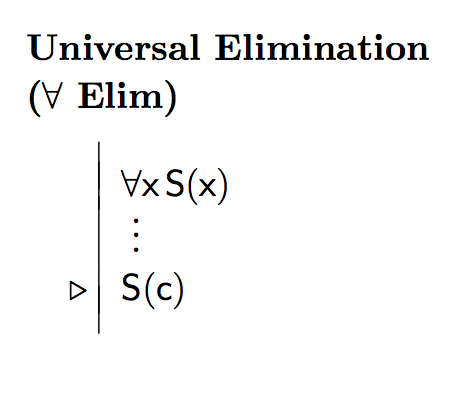
\includegraphics[scale=0.3]{img/rule_universal_elim.png}
\end{center}
\vfill


%--- end paste
%--------------- 
 


\end{multicols*}

\end{document}